\section{Introduction}
\blfootnote{This work was funded by the ANR Project SAROUMANE (ANR-22-CE23-0011) and by the European Union (ERC, HI-Audio, 101052978). Views and opinions expressed are however those of the author(s) only and do not necessarily reflect those of the European Union or the European Research Council. Neither the European Union nor the granting authority can be held responsible for them.}

%%%% General section of audio generation
In the era of deep learning, generating high-fidelity audio data is a major research topic for improving the performance of machine listening algorithms.
Apart from audio synthesis for listening applications, it can also be seen as an important asset for data augmentation in unbalanced settings, such as in sound event detection, speech processing, or music information retrieval-related tasks.  


%%%% examples of famous deep audio generation systems
Speech generation has witnessed the utilization of various architectures and input methods to produce high-quality audio speech.
Notable algorithms in speech generation encompass text-to-speech (TTS) variational autoencoder \cite{lu21d_interspeech}, as well as convolutional neural network (CNN) architectures operating directly on raw audio %input 
such as Wavenet \cite{vanwavenet}. 
Mel spectrograms serve as an alternative input for speech generation, with such examples as Waveglow \cite{prenger2019waveglow}, based on normalizing flow \cite{rezende2015variational}, and HiFi-GAN \cite{kong2020hifi}, based on a generative adversarial network (GAN) \cite{goodfellow2014generative}. 
 

Diffusion models \cite{ho2020denoising, song2021scorebased} have recently emerged as highly advanced deep generative models where a stochastic flow to solve differential equations is governed by a fixed noise schedule.
They have surpassed the long-standing dominance of  GANs in the field of image synthesis \cite{huang2018introduction, liu2020generative, dhariwal2021diffusion}.
Diffusion models have also been considered for various speech-related tasks such as speech enhancement \cite{lemercier2023storm, richter2023speech, lu2022conditional} or speech separation \cite{scheibler2023diffusion, chen2023sepdiff}.
Diffusion-based speech generation methods that use conditioning on mel spectrograms have also been proposed, notably Wavegrad \cite{chen2020wavegrad} and DiffWave \cite{kong2020diffwave}. Building upon DiffWave,  PriorGrad \cite{lee2021priorgrad} replaces the standard Gaussian prior noise assumption by an adaptive prior, while SpecGrad \cite{koizumi2022specgrad} applies constraints to ensure the time-varying spectral envelope aligns with the log-mel spectrogram. 

Nonetheless, diffusion models face an ongoing challenge in efficient training. Their stability relies heavily on large datasets to ensure the stability of the diffusion process through the iterations \cite{wang2023patch}.
An essential component is the noise schedule governing the reverse process for generating speech. Recent advances such as FastDiff \cite{huang2022fastdiff} propose to predict the noise schedule dynamically throughout iterations to reduce their number and enhance the signal generation.
Furthermore, the versatility of speech signals presents domain adaptation limitations with a diffusion model framework \cite{farahani2020brief}. These limitations result in poor generalization 
% to a wide array of real-world waveform data
to unseen speakers in speech generation scenarios.

Our paper addresses the latest drawback which, to the best of our knowledge, has not been explored within the diffusion model framework for speech generation. In this article, we introduce a straightforward extension to WaveGrad, aiming to rectify conditioning errors on the mel spectrogram during the reverse process iterations. 
As illustrated in Fig.~\ref{fig:method}, we use the Griffin-Lim algorithm (GLA)  \cite{griffin1984signal} to partially reconcile the phase of the short-time Fourier transform of the current sample in the diffusion process with the magnitude spectrogram obtained as pseudo-inverse of the conditioning mel spectrogram.
Our objective is to ensure consistency in the reverse  process, even when the user-provided signal significantly differs from those in the training set.


\begin{figure}[t]
\centering
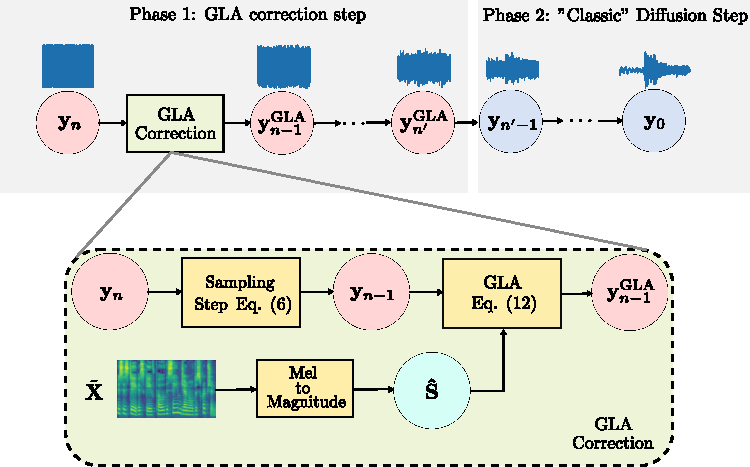
\includegraphics[width=0.98\columnwidth]{figs/GLA-Grad.pdf}
\caption{Griffin-Lim corrected diffusion model}
\vspace{-.3cm}
\label{fig:method}
\end{figure}

The achieved scores demonstrate GLA-Grad's competitiveness with WaveGrad and SpecGrad when using a single-speaker dataset.
However, GLA-Grad significantly outperforms them as the dataset's speaker count increases, highlighting its superior generalization capability across multiple speakers.
Additionally, experiments involving unseen speakers during training demonstrate GLA-Grad's effectiveness in addressing domain adaptation challenges.
